\chapter{Parte teórica y desarrollo del código}
El paquete \texttt{solaR2} toma como marco teórico el libro de Oscar Perpiñán, tutor de este trabajo, Energía Solar Fotovoltaica \cite{Perpinan2023} para cada una de las operaciones de cálculo que realizan cada una de las funciones.
En la figura \ref{fig:orge0cb772}, se muestra un diagrama que resume los pasos que se siguen a la hora de calcular la producción de sistemas fotovoltaicos.
\begin{figure}[p]
\centering
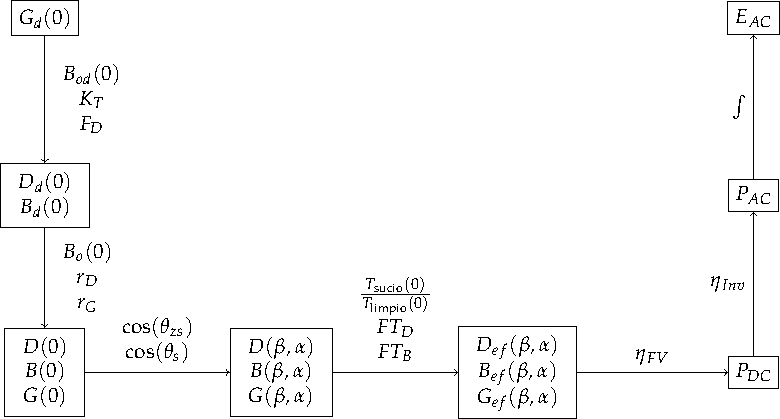
\includegraphics[keepaspectratio,width=0.9\textwidth,height=0.5\textheight]{figuras/ProcedimientoCalculoRadiacionInclinada.pdf}
\caption{\label{fig:orge0cb772}Procedimiento de cálculo}
\end{figure}
Estos pasos son:
\begin{enumerate}
\item Obtener la irradiación global diaria en el plano horizontal
\item A partir de la irradiación global, obtener las componentes de difusa y directa.
\item Se trasladan estos valores de irradición a valores de irradiancia.
\item Con estos valores se pueden obtener los valores correspondientes en el plano del generador
\begin{enumerate}
\item Sin los efectos de la suciedad de los modulos y las sombras que se generan unos con otros.
\item Con estos efectos
\end{enumerate}
\item Integrando estos valores se pueden obtener las estimaciones irradiación diaria difusa, directa y global
\item El generador fotovoltaico produce una potencia en corriente continua dependiente del rendimiento del mismo..
\item Se transforma en potencia en corriente alterna mediante un inversor que tiene una eficiencia asociada.
\item Integrando esta potencia se puede obtener la energía que produce el generador en un tiempo determinado.
\end{enumerate}

\section{Naturaleza de la radiación solar}
\label{sec:orgb9df69c}
Para el cálculo de la radiación solar que incide en una superficie se deben distinguir tres componentes diferenciados:
\begin{itemize}
\item \textbf{Radiación Directa}, B\nomenclature[B]{\(B\)}{Radiación directa}: porción de radiación que procede en línea recta desde el Sol.
\item \textbf{Radiación Difusa}, D\nomenclature[D]{\(D\)}{Radiación difusa}: fracción de radiación que procede de todo el cielo, excepto del Sol. Son todos aquellos rayos que dispersa la atmósfera.
\item \textbf{Radiación del albedo}, R\nomenclature[R]{\(R\)}{Radiación del albedo}: parte de la radiación procedente de la reflexión con el suelo.
\end{itemize}
La suma de las tres componentes constituye la denominada radiación global: \nomenclature[G]{\(G\)}{Radiación global}
\begin{equation}
G = B + D + R
\label{eq:comp_rad}
\end{equation}
Tomando como base el libro antes mencionado \cite{Perpinan2023}, se describirá el proceso que se ha de seguir para obtener una estimación de las componenetes directa y difusa a partir del dato de radiación global, dado que es el que comúnmente se puede obtener de una localización determinada.

\subsection{Radiación fuera de la atmósfera terrestre}
\label{sec:org89250ce}
Lo primero que se menciona en dicho proceso es la obtención de la irradiancia denominda extra-terrestre o extra-atmosférica, que es la radiación que llega a la atmósfera, directamente desde el Sol, que no sufre ninguna pérdida por interaccionar con algún medio. Como la relación entre el tamaño de nuesto plenta y la distancia entre el Sol y la Tierra es muy reducida, es posible asumir que el valor de dicha irradiancia es constante, siendo este valor \(B_0=1367\frac{W}{m^2}\), según varias mediciones.
Como la órbita que describe la Tierra alrededor del Sol no es totalmente circular, sino que tiene forma de elipse, para calcular la irradiancia incidente en una superficie tangente a la atmosfera en ua latitud concreta, debemos aplicar un facot de correción de la excentricidad de la elipse:
\begin{equation}
B_0(0)=B_0\epsilon_0cos\theta_{zs}
\label{eq:irrad_horiz}
\end{equation}
Siendo cada componente:
\begin{itemize}
\item Irradiancia extra-terrestre: \(B_0=1367\frac{W}{m^2}\) \nomenclature[B0]{\(B_0\)}{Irradiancia extra-atmosférica o extra-terrestre}
\item Factor de corrección por excentricidad: \(\epsilon_0=(\frac{r_0}{r})^2=1+0.033\cdot cos(\frac{2\pi d_n}{365})\)\footnote{Para las ecuaciones de este apartado se va a optar por poner la ecuación más simple posible. Sin embargo, el paquete \texttt{solaR2} otorga la posibilidad de realizar los cálculos de utilizando las ecuaciones propuestas por 4 autores diferentes.} \nomenclature[epsilon0]{\(\epsilon_0\)}{Corrección debida a la excentricidad de la elipse de la trayectoria terrestre alrededor del sol}
\item Ángulo zenital solar: \(cos(\theta_{zs})=cos(\delta)cos(\omega)cos(\phi)+sin(\delta)+sin(\phi)\)\footnote{Se van a utilizar las ecuaciones propuestas por P.I. Cooper \cite{Cooper1969} por su simpleza.} \nomenclature[thetazs]\{\(\theta_{zs}\)\}\{Ángulo cenital solar\}

Donde:
\begin{itemize}
\item Declinación: \(\delta =23,45º\cdot sin(\frac{2\pi \cdot (d_n+284)}{365})\) \nomenclature[delta]{\(\delta\)}{Declinación}
\item Latitud: \(\phi\) \nomenclature[phi]{\(\phi\)}{Latitud}
\item Hora solar o tiempo solar verdadero: \(\omega = 15\cdot (TO-AO-12)+\Delta \lambda +\frac{EoT}{4}\) \nomenclature[omega]{\(\omega\)}{Hora solar o tiempo solar verdadero}

Donde:
\begin{itemize}
\item Hora oficial: \(TO\) \nomenclature[TO]{\(TO\)}{Hora oficial}
\item Adelanto oficial durante el horario de verano: \(AO\) \nomenclature[AO]{\(AO\)}{Adelanto oficial durante el horario de verano}
\item Diferencia entre la longitud local y la longitud del huso horario: \(\Delta \lambda\) \nomenclature[deltalambda]{\(\Delta \lambda\)}{Diferencia entre la longitud local y la longitud del huso horario}
\item Ecuación del tiempo: \(EoT=229,18\cdot (-0,0334\cdot sin(\frac{2\pi}{365,24}\cdot dn)+0,04184\cdot sin(2\cdot \frac{2\pi}{365,24}\cdot dn+3,5884))\) \nomenclature[EoT]{\(EoT\)}{Ecuación del tiempo}
\end{itemize}
\end{itemize}
\end{itemize}

Esta irradiancia extra-terrestre solo tiene componentes geométicas. De modo que, si integramos la ecuación \ref{eq:irrad_horiz}, se obtiene la irradiación diaria extra-terrestre:
\begin{equation}
B_{0d}(0)=-\frac{T}{\pi}B_0\epsilon_0(\omega_s sin\phi sin\delta + cos\phi cos\delta sin \omega_s)
\label{eq:irrad_dia}
\end{equation}
Siendo:
\begin{itemize}
\item Ángulo del amananecer: \nomenclature[omegas]{\(\omega_s\)}{Ángulo del amanecer}
\[
  \omega_s=\begin{cases}
  -\arccos(-\tan\delta\tan\phi)& \text{si $|\tan\delta\tan\phi|<1$}\\
  -\pi& \text{si $-\tan\delta\tan\phi<-1$}\\
  0& \text{si $-\tan\delta\tan\phi>1$}
  \end{cases}\]
\end{itemize}

Es posible demostrar que el promedio mensual de esta irradiación diaria coincide numéricamente con el valor de irradiación diaria correspondiente a los denominados ``días promedios'', días en los que la declinación correpondiente coincide con el promedio mensual (tabla \ref{tab:DiasPromedio})
\begin{center}
{\footnotesize }%
\begin{table}[h]
{\footnotesize \caption{Valor $d_{n}$ correspondiente a los doce días promedio.\label{tab:DiasPromedio}}
}{\footnotesize \par}

\centering{}{\footnotesize }\begin{tabular}{>{\centering}p{6mm}>{\centering}m{4mm}>{\centering}m{4mm}>{\centering}m{4mm}>{\centering}m{4mm}>{\centering}m{4mm}>{\centering}m{4mm}>{\centering}m{4mm}>{\centering}m{4mm}>{\centering}m{4mm}>{\centering}m{4mm}>{\centering}m{4mm}>{\centering}m{3mm}}
\toprule 
{\footnotesize Mes} & {\footnotesize Ene} & {\footnotesize Feb} & {\footnotesize Mar} & {\footnotesize Abr} & {\footnotesize May} & {\footnotesize Jun} & {\footnotesize Jul} & {\footnotesize Ago} & {\footnotesize Sep} & {\footnotesize Oct} & {\footnotesize Nov} & {\footnotesize Dic}\tabularnewline
\midrule
$d_{n}$ & {\footnotesize 17} & {\footnotesize 45} & {\footnotesize 74} & {\footnotesize 105} & {\footnotesize 135} & {\footnotesize 161} & {\footnotesize 199} & {\footnotesize 230} & {\footnotesize 261} & {\footnotesize 292} & {\footnotesize 322} & {\footnotesize 347}\tabularnewline
\bottomrule
\end{tabular}
\end{table}

\par\end{center}{\footnotesize \par}

\subsection{Cálculo de componentes de radiación solar}
\label{sec:org4603e3a}
Para caracterizar la radiación solar en un lugar, Liu y Jordan \cite{Liu.Jordan1960} propusieron el índice de claridad, \(K_T\). Este índice es la relación entre la radiación global y la radiación extra-atmosférica, ambas en el plano horizontal. El índice de claridad diario es la relación entre los valores diarios de irradiación: \nomenclature[KT]{\(K_T\)}{Índice de claridad} \nomenclature[KTd]\{\(K_{Td}\)\}\{Índice de claridad diario\}
\begin{equation}
K_{Td}=\frac{G_d(0)}{B_{0d}(0)}
\label{eq:ind-cla-dia}
\end{equation}
mientras que el índice de claridad mensual es la relación entre las medias mensuales de la irradiación diaria: \nomenclature[KTm]\{\(K_{Tm}\)\}\{Índice de claridad mensual\}
\begin{equation}
K_{Tm}=\frac{G_{d,m}(0)}{B_{0d,m}(0)}
\label{eq:ind-cla-men}
\end{equation}

Una vez se tiene el índice de claridad, se puede calcular la fracción de radiación difusa en el plano horizontal. En el caso de medias mensuales \cite{Page1961}:
\begin{equation}
F_{Dm}=1-1,13\cdot K_{Tm}
\end{equation}
Donde:
\begin{itemize}
\item Fracción de radiación difusa: \(F_D=\frac{D(0)}{G(0)}\) \nomenclature[FD]{\(F_D\)}{Fracción de difusa} \nomenclature[FDd]\{\(F_{Dd}\)\}\{Fracción de difusa diaria\} \nomenclature[FDm]\{\(F_{Dm}\)\}\{Fracción de difusa mensual\}
\end{itemize}

Al tener la fracción de radiación difusa, se pueden obtener los valores de la radiación directa y difusa en el plano horizontal:
\begin{equation}
D_d(0)=F_D\cdot G_d(0)
\label{dif-rad}
\end{equation}
\begin{equation}
B_d(0)=G_d(0)-D_d(0)
\label{dif-rad}
\end{equation}

\section{Operaciones del paquete \texttt{solaR2}}
\label{sec:org8e7bbac}
En la figura \ref{fig:org2cb1708}, se muestra el proceso de cálculo que sigue el paquete a la hora de obtener la estimación de la producción del sistema fotovoltaico.
\begin{figure}[p]
\centering
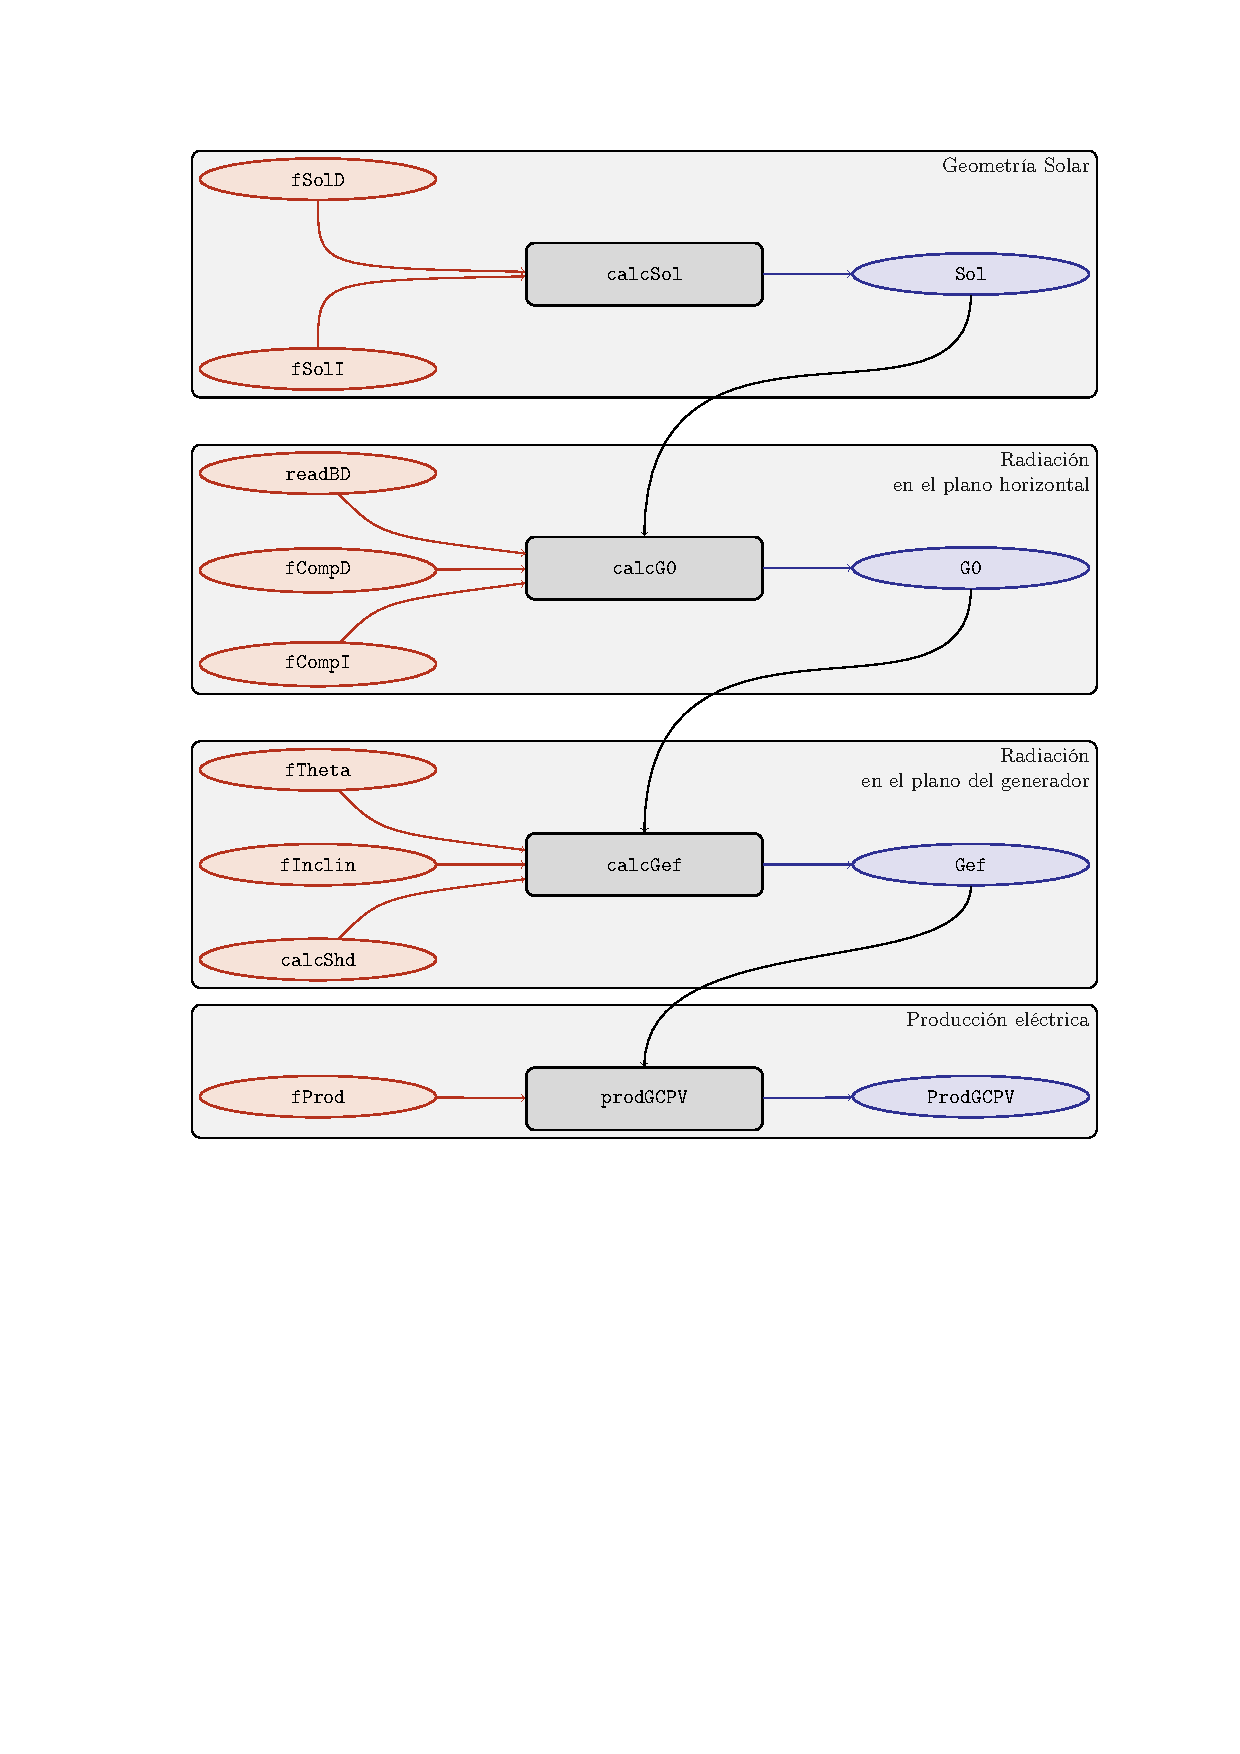
\includegraphics[keepaspectratio,width=0.9\textwidth,height=0.5\textheight]{figuras/procedure.pdf}
\caption{\label{fig:org2cb1708}Proceso de cálculo de las funciones de \texttt{solaR2}}
\end{figure}
A la hora de estimar la producción, el programa sigue los siguientes procesos:
\begin{enumerate}
\item Se calcula la geometría que definen la posición de la Tierra frente al Sol.
\begin{enumerate}
\item Mediante la función fSolD, se calcula:
\begin{itemize}
\item El ángulo de declinación de la Tierra (\(\delta\)).
\item La corrección debida a la excentricidad de la elipse de la trayectoria terrestre alrededor del sol (\(\epsilon_0\)).
\item La ecuación del tiempo (\(EoT\)).
\item El ángulo del amanecer
\end{itemize}
\item Mediante la función fSolI, se calcula:
\begin{itemize}
\item La hora solar (\(\omega\)).
\item El momento del día en el que es de noche.
\item El ángulo zenital solar (\(\theta_{zs}\)).
\item El ángulo de altura solar (\(\gamma_s\).
\item El ángulo azimutal solar (\(\psi_s\)).
\item La irradiancia extra-terrestre en el plano horizontal (\(B_0(0)\)).
\end{itemize}
\item El resultado de ambas funciones se juntan en un solo objeto de clase \texttt{Sol} mediante la función calcSol.
\end{enumerate}
\item Se estima la radiación en el plano horizontal.
\begin{enumerate}
\item La información de irradiación en el plano horizontal (en todos sus componentes o, en su defecto, solo la global(\(G_d(0)\))) y temperatura viene dada en un objeto de clase \texttt{Meteo}.
\item Mediante la función fCompD, se calcula:
\begin{itemize}
\item La fracción de radiación difusa diaria (\(F_{Dd}\)).
\item El índice de claridad diario (\(K_{Td}\)).
\item Si solo se tienen datos de la componente global de irradición:
\begin{itemize}
\item La irradiación directa en el plano horizontal (\(B_d(0)\)).
\item La irradiación difusa en el plano horizontal (\(D_d(0)\)).
\end{itemize}
\end{itemize}
\item Mediante la función fCompI, se calcula:
\begin{itemize}
\item La fracción de radiación difusa (\(F_D\)).
\item El índice de claridad (\(K_T\)).
\item Si solo se tienen datos de la componenete global de irradiancia (\(G(0)\)):
\begin{itemize}
\item La irradiancia directa en el plano horizontal (\(B(0)\)).
\item La irradiancia difusa en el plano horizontal (\(D(0)\)).
\end{itemize}
\end{itemize}
\item El resultado de ambas funciones junto a medias mensuales y valores anuales se consolidan en un solo objeto de clase \texttt{G0} (que incluye los objetos \texttt{Sol} y \texttt{Meteo} de los que parte) mediante la función calcG0.
\end{enumerate}
\item Se estima la radiación en el plano del generador.
\begin{enumerate}
\item La información de radiación puede venir dada en forma de un objeto de clase \texttt{Meteo} o un objeto de clase \texttt{G0} (ya que es este último el que se necesita para estimar la radiación en el plano del generador).
\item Mediante la función fTheta, se calcula:
\begin{itemize}
\item Ángulo de inclinación de la superficie del módulo (\(\beta\)).
\item Ángulo azimutal de la superficie del módulo (\(\alpha\) ).
\item Ángulo de incidencia de la irradiancia solar en la superficie del módulo (\(\theta_s\)).
\end{itemize}
\item Mediante la función fInclin, se calcula:
\begin{itemize}
\item La irradiancia extra-terrestre en la superficie inclinada (\(B_0(\beta, \alpha)\)).
\item La irradiancia directa normal (\(B(n)\)).
\item Las irradiancias global (\(G(\beta, \alpha)\)), directa (\(B(\beta, \alpha)\)), difusa (\(D(\beta, \alpha)\))(total, isotropica y anisotrópica) y del albedo (\(R(\beta, \alpha)\)) sobre una superficie inclinada.
\item Las irradiancias efectivas global (\(G_{ef}(\beta, \alpha)\)), directa (\(B_{ef}(\beta, \alpha)\)), difusa (\(D_{ef}(\beta, \alpha)\))(total, isotropica y anisotrópica) y del albedo (\(R_{ef}(\beta, \alpha)\)) sobre una superficie inclinada.
\item Los factores de pérdidas angulares para las componentes directa (\(FT\)), difusa (\(FT_D\)), y del albedo (\(FT_R\)).
\end{itemize}
\item Mediante la función calcShd, se puede calcular:
\begin{itemize}
\item La irradiancia e irradiación incluyendo sombras para seguidores a dos ejes y horizontales y paneles fijos mediante la función fSombra.
\end{itemize}
\item El resultado de estas funciones junto a medias mensuales y valores anuales se consolidan en un solo objeto de clase \texttt{Gef} (que incluye el objeto \texttt{G0} del que parte) mediante la función calcGef.
\end{enumerate}
\item Se estima la producción eléctrica.
\begin{enumerate}
\item Mediante la función fProd, se calcula:
\begin{itemize}
\item La potencia en corriente continua (\(P_{DC}\)).
\item La potencia en corriente alterna (\(P_{AC}\).
\end{itemize}
\item Estos resultados, llevados a valores diarios, mensuales y anuales, se pueden convertir en valores de energía (\(E_{DC}\) y \(E_{AC}\)) y de productividad del sistema (\(Y_f\)), los cuales se consolidan en un solo objeto de clase \texttt{ProdGCPV} (que incluye el objeto \texttt{Gef} del que parte) mediante la función prodGCPV.
\end{enumerate}
\end{enumerate}
